\subsubsection*{Express Lane Check-in}
The ‘Express Check-in Toll Lane’-component, seen in \autoref{fig:life_cycle_statemachine_toll_lane_computer_express_check_in}, receives a message from the antenna to indicate that a vehicle with a toll tag has entered the lane. It reacts by sending a message to the station server to check that the tag is valid. If it receives true it tells the station server to check in the tag, opens the barrier, then closes it when the antenna informs it that the tag can no longer be detected.  Otherwise it goes to a faulty tag state and waits for a cashier to resolve the situation. 
\begin{figure}[H]
\centering
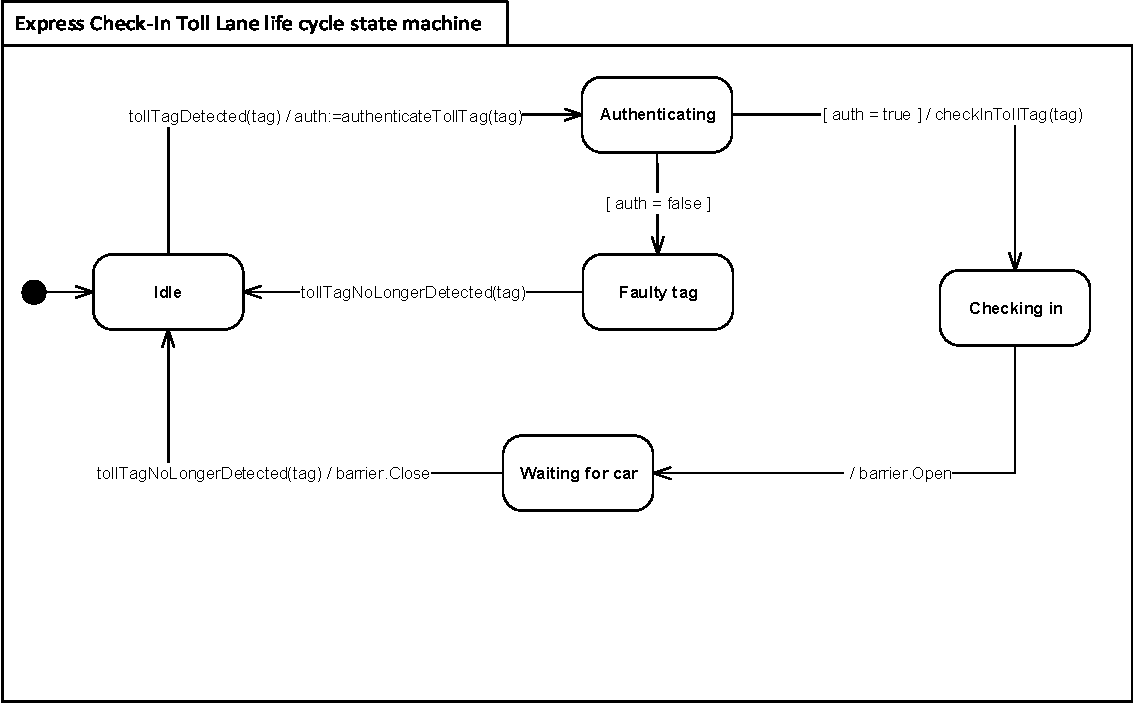
\includegraphics[width=0.7\linewidth]{img/protocol_state_machine/life_cycle_statemachine_toll_lane_computer_express_check_in.png}
\caption{The life-cycle state machine for express lane check-in}
\label{fig:life_cycle_statemachine_toll_lane_computer_express_check_in}
\end{figure}

\subsubsection*{Express Lane Check-out}
The ‘Express Check-out Toll Lane’-component, seen in \autoref{fig:life_cycle_statemachine_toll_lane_computer_express_check_out}, receives a message from the antenna to indicate that a vehicle with a toll tag has entered the lane. It reacts by sending a message to the station server to check that the tag is checked in. If it receives true it tells the station server to check out the tag, opens the barrier, then closes it when the antenna informs it that the tag can no longer be detected.  Otherwise it goes to a faulty tag state and waits for a cashier to resolve the situation. 
\begin{figure}[H]
\centering
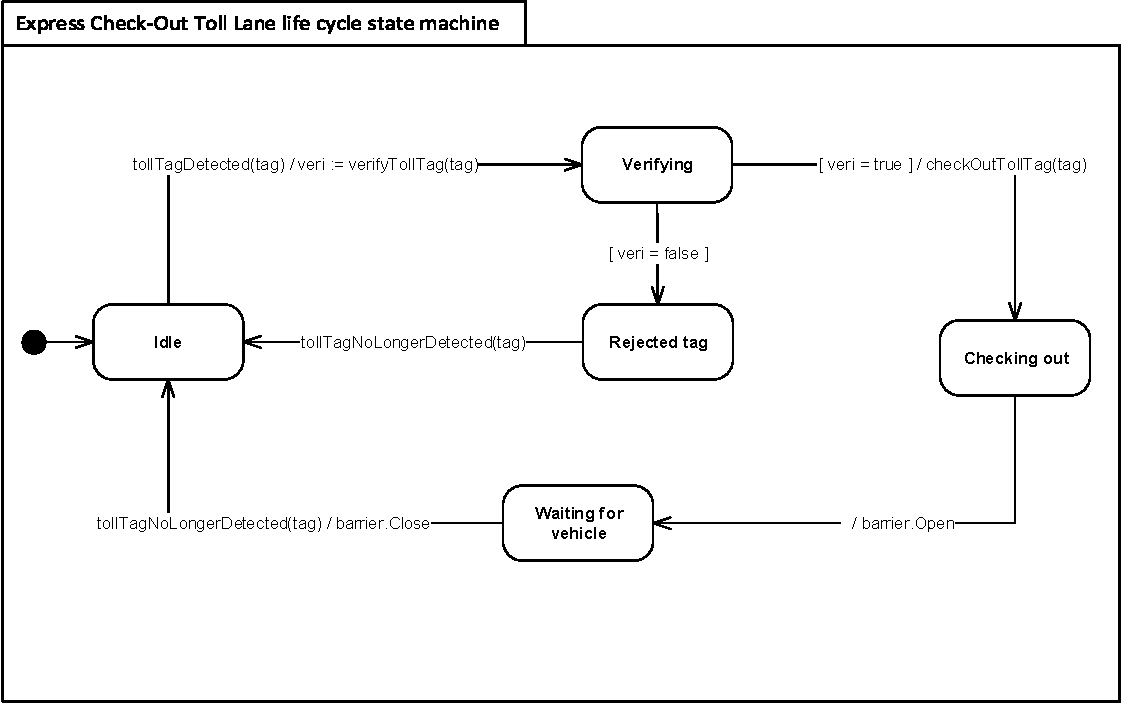
\includegraphics[width=0.7\linewidth]{img/protocol_state_machine/life_cycle_statemachine_toll_lane_computer_express_check_out.png}
\caption{The life-cycle state machine for express lane check-out}
\label{fig:life_cycle_statemachine_toll_lane_computer_express_check_out}
\end{figure}

\subsubsection*{Normal Lane Check-in}
The ‘Normal Check-in Toll Lane’-component, seen in \autoref{fig:life_cycle_state_machine_toll_lane_computer}, waits for the touch screen to send information about a vehicle. It returns the price for that vehicle, then waits to receive payment via cash or credit card. If payment is received via card, it contacts the bank about the transaction. It then prints a ticket and opens the barrier long enough for the customer to pass.
\begin{figure}[H]
\centering
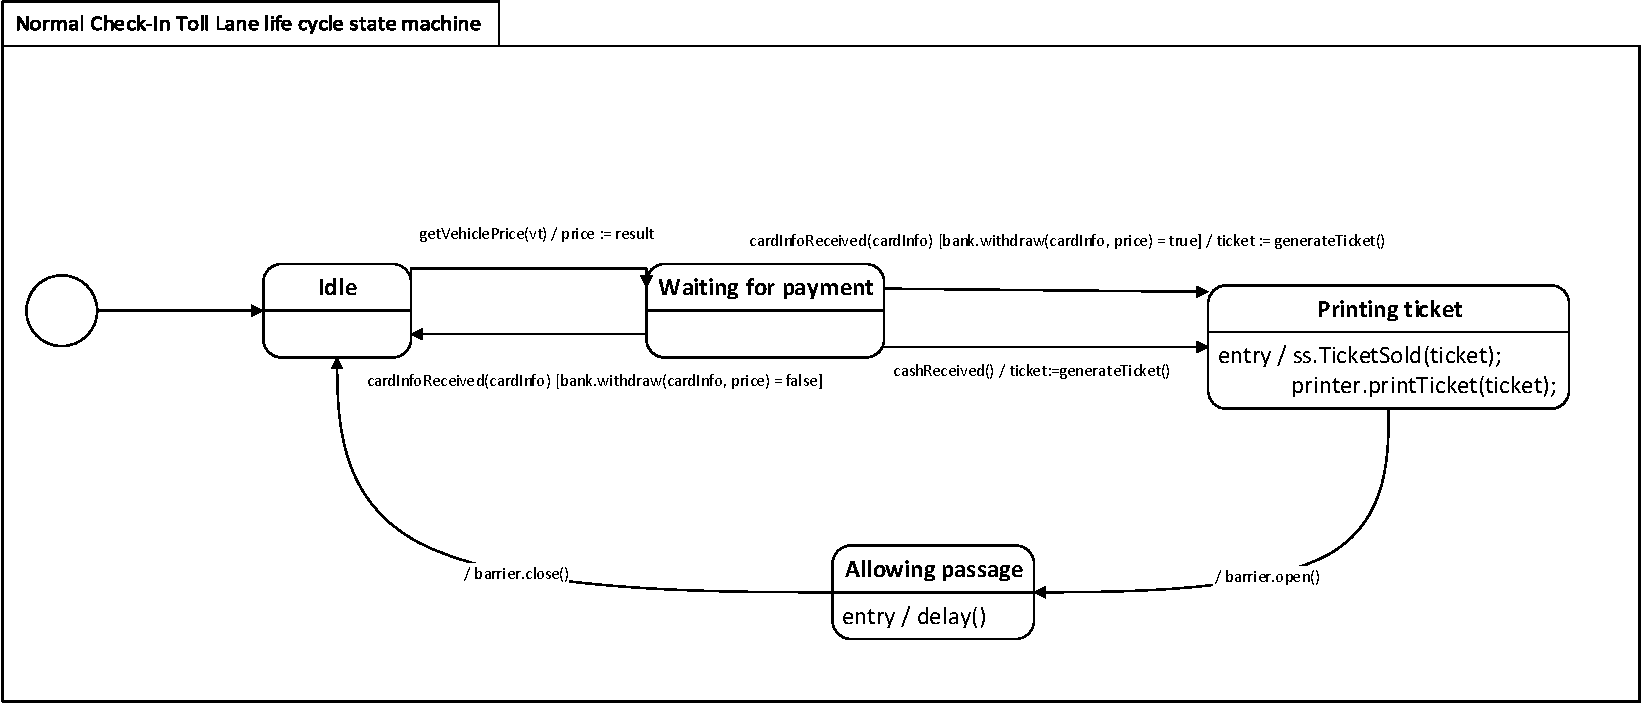
\includegraphics[width=0.7\linewidth]{img/protocol_state_machine/life_cycle_state_machine_toll_lane_computer.png}
\caption{The life-cycle state machine for normal lane check-in}
\label{fig:life_cycle_state_machine_toll_lane_computer}
\end{figure}

\subsubsection*{Normal Lane Check-out}
The ‘Normal Check-out Toll Lane’-component, seen in \autoref{fig:life_cycle_state_machine_toll_computer_normal_lane}, waits for a ticket to be inserted. When it is, it contacts the station server to validate the ticket. If the ticket is valid, it opens the barrier, waits for the customer to leave, then closes the barrier. Otherwise it goes to an invalid ticket state and waits for a cashier to resolve the situation.
\begin{figure}[H]
\centering
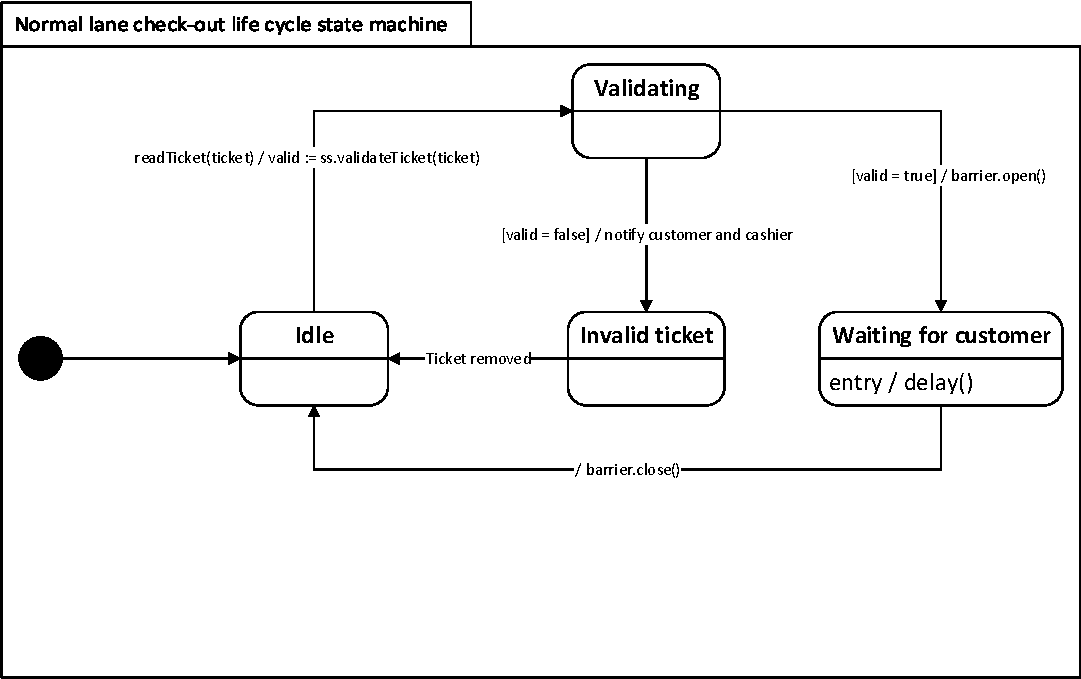
\includegraphics[width=0.7\linewidth]{img/protocol_state_machine/life_cycle_state_machine_toll_computer_normal_lane.png}
\caption{The life-cycle state machine for express lane check-out}
\label{fig:life_cycle_state_machine_toll_computer_normal_lane}
\end{figure}

\subsubsection*{Station server}
The ‘Station server’-component, seen in \autoref{fig:life_cycle_state_machine_station_server}, sends messages between the Toll Lane and the Enterprise Server.
\begin{figure}[H]
\centering
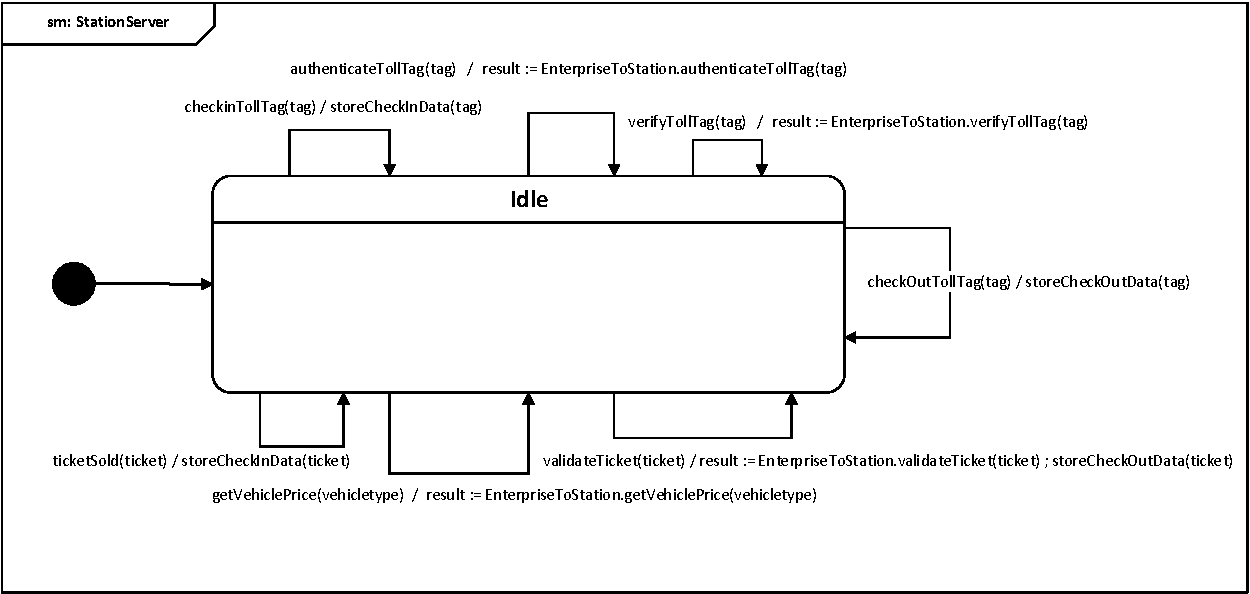
\includegraphics[width=0.7\linewidth]{img/protocol_state_machine/life_cycle_state_machine_station_server.png}
\caption{The life-cycle state machine for express lane check-out}
\label{fig:life_cycle_state_machine_station_server}
\end{figure}


\subsubsection*{Enterprise server}